\chapter{緒論}
\fontsize{12pt}{18pt}\selectfont

% ------------------------- 1.1 ------------------------- %
\section{前言}
% 人體動作模擬發展;應用
在科技日益發展下,人類的生理資訊不侷限於臨床醫學的探討,電腦模擬與分析已成為現今生物醫學領域的重要研究方向之一 \cite{roupa2022modeling} \cite{uhlrich2023ten},
在技術不斷提升的情況下,使我們能夠更全面和深入地瞭解人體的生理狀況、生物力學等表現,例如通過運動模擬來研究運動員,
分析在訓練中的姿勢、肌肉和關節受力情況,來改善訓練過程與制定訓練菜單 \cite{barnamehei2020muscle} \cite{bullock2022just},
此外電腦模擬在醫學領域中有著廣泛的應用,例如協助醫生制定更有效的治療方法,或是通過模擬手術來研究手術風險和效果 \cite{delp1990interactive} \cite{rajagopal2020pre}。
綜合上述,在人體模擬和分析的發展,不僅提供了更多的生理資訊與科學研究方法,同時也為人類的健康帶來了正面影響。

% 人體動作模擬種類
在人體動作模擬與分析中,本文作者將其分為三大領域,如圖 \ref{ch1_fig_StudyBackground} 所示,
包含著人體運動學、動力學與肌肉動力學,每個領域所感興趣的資訊、所需的量測設備皆不相同,唯獨共同點是需要一個模型,
才能進行後續的模擬與分析。

\begin{figure}[!ht]
	\centering
	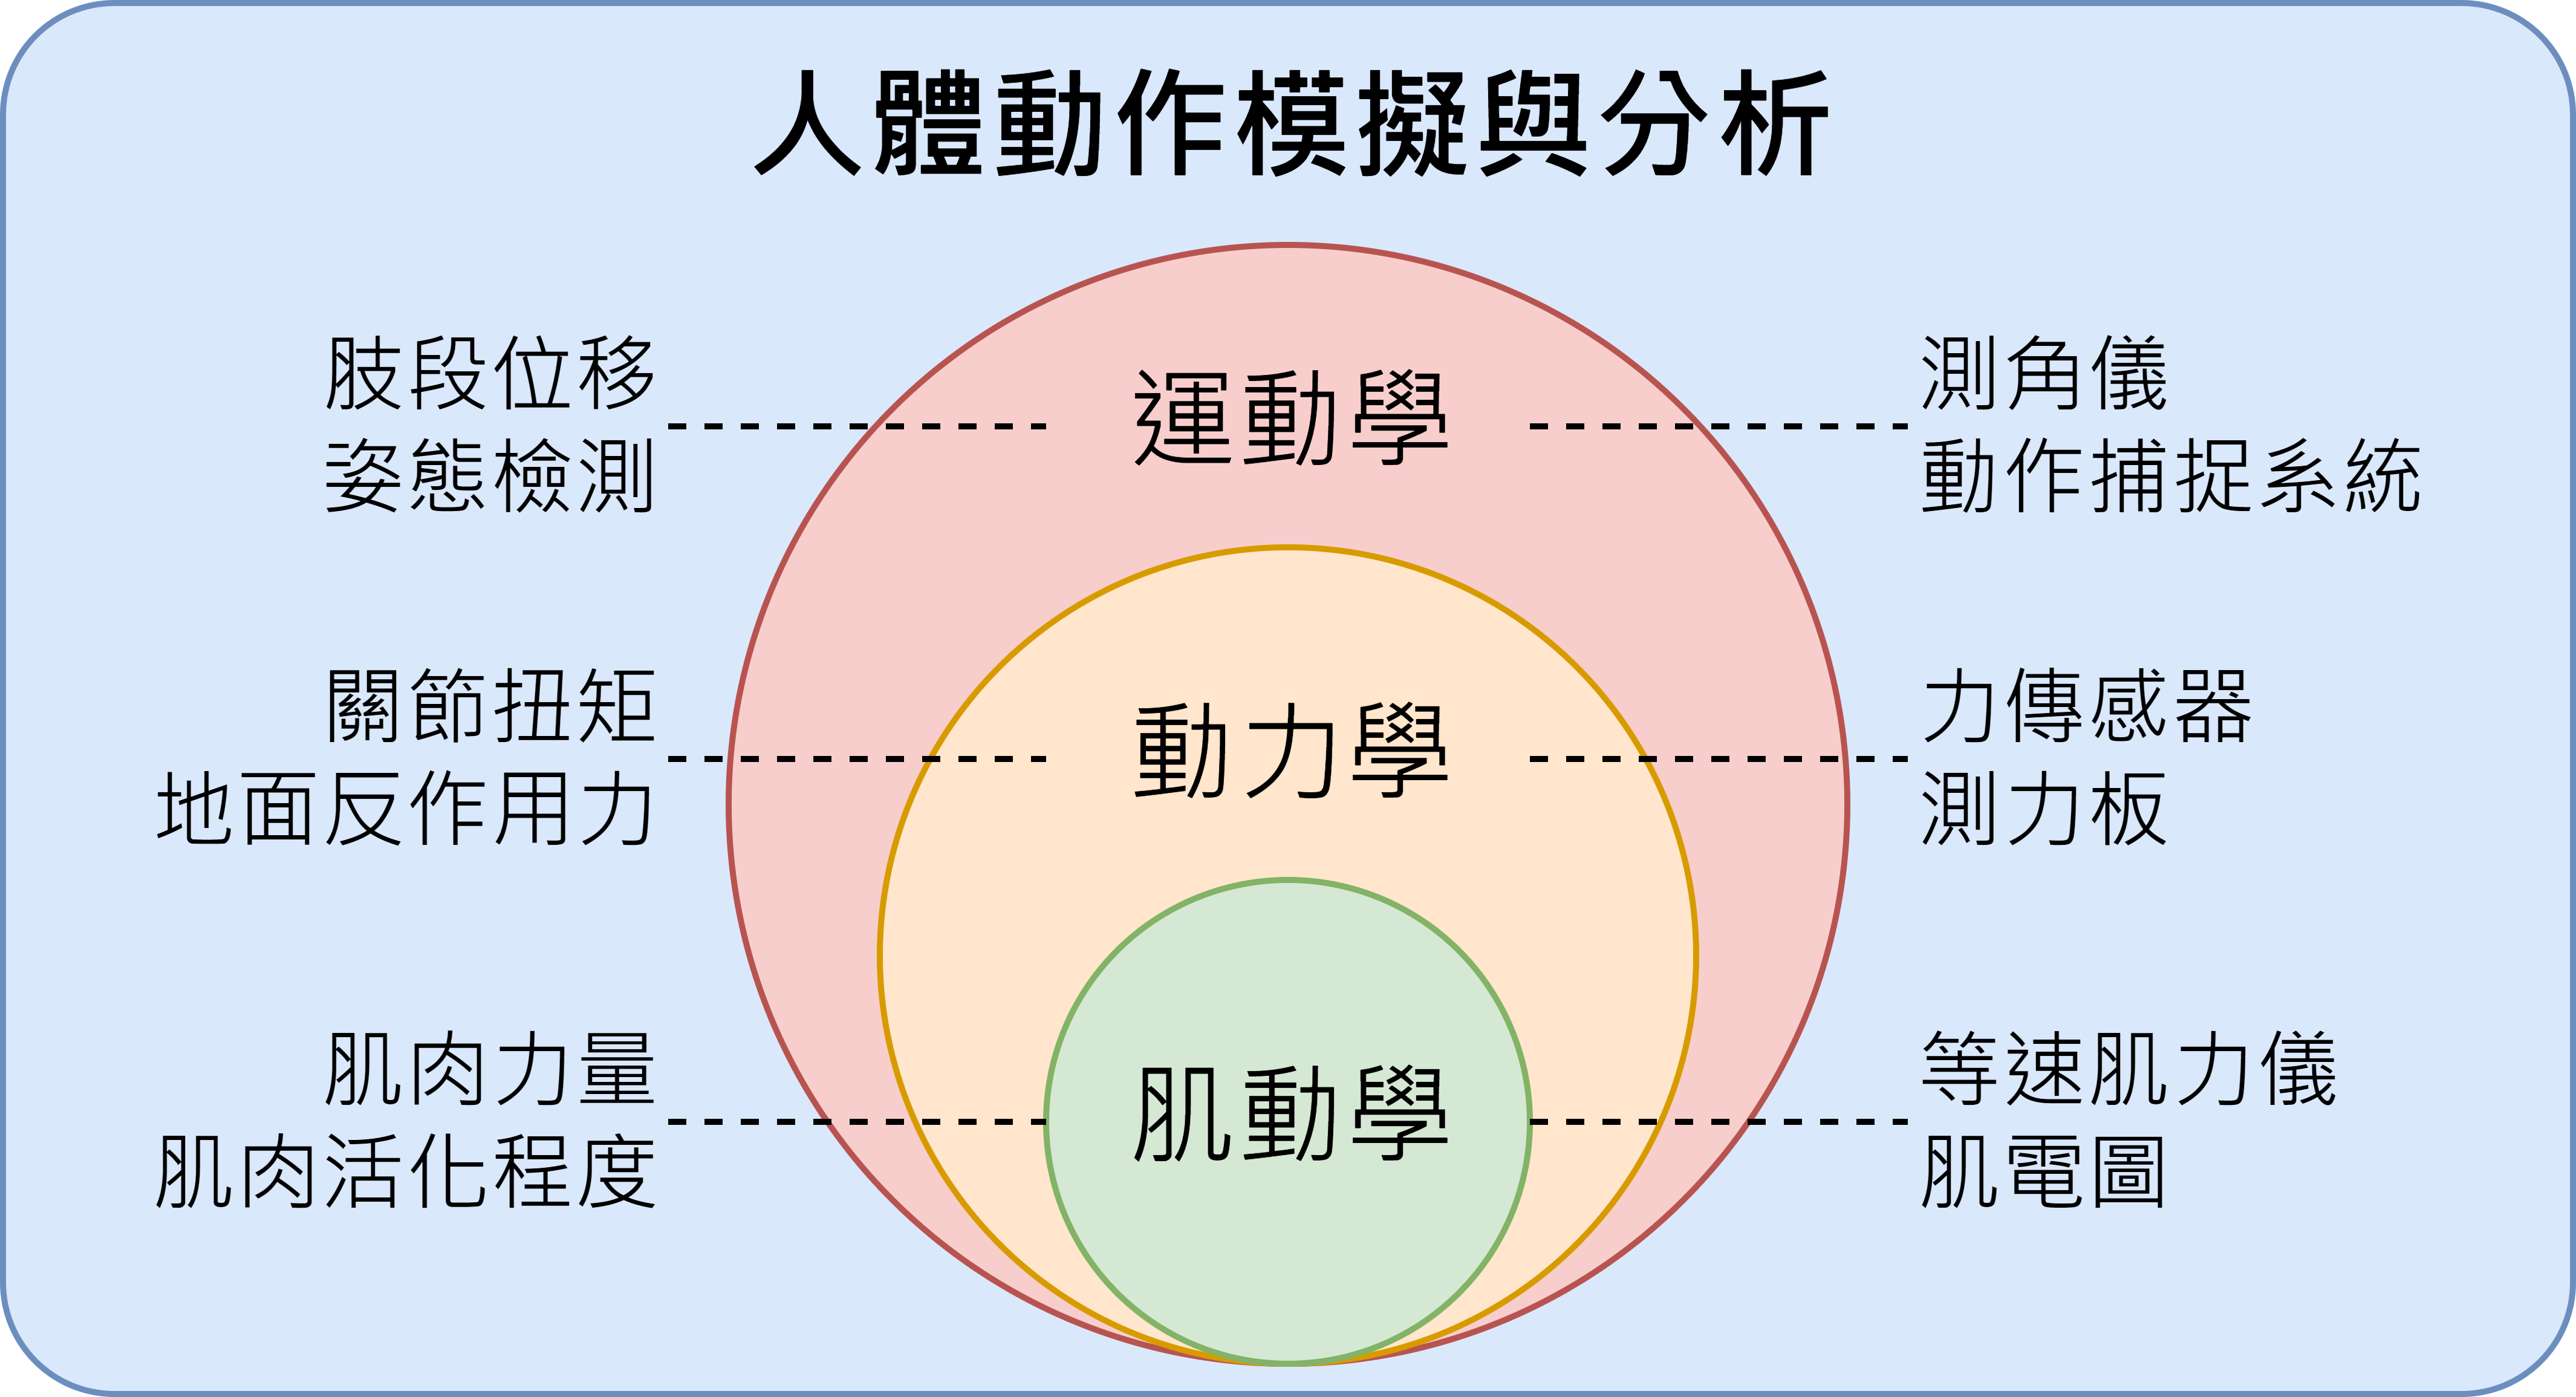
\includegraphics[width=12cm]{figure/ch1_fig_StudyBackground.png}
    \caption[人體動作模擬與分析之種類劃分]{人體動作模擬與分析之種類劃分}
    \label{ch1_fig_StudyBackground}
\end{figure}

% 模型選擇;通用模型;個人化模型
模型的挑選上,可以選擇以大眾生理資訊所建立的通用模型,該模型並不代表任何一個人,
但可藉由適當地縮放來代表受試者、進行後續作業 \cite{winby2008evaluation},通用模型的優點是無需繁雜的模型建立過程,
簡易的調整即可使用,但相對地缺點就是該模型的準確度低,使得模擬與分析結果並不能完整的體現該受試者的生理結果,
尤其若當應用領域在於復健、運動訓練上,這些生理資訊的結果佔了舉足輕重的角色,故在個人化模型的建立上是必然的 \cite{akhundov2022subject}。
個人化模型乃是針對個體的解剖學、生理學和生物力學等資訊,來量身打造的模擬模型,其提供更加精準和特定的資訊,
從而徹底改變復健和運動科學領域 \cite{pizzolato2017bioinspired}。 

% ------------------------- 1.2 ------------------------- %
\section{研究動機與目的}
% Vicon 骨架取代
% 時間軸對齊方式
近年在新型冠狀病毒 (COVID-19) 的肆虐下,世界各地的醫療與復健服務產生了重大影響,除了原先的各種疾病治療外,
還要積極治癒相關染疫者,其對於醫院和診所不堪重負,而防止疫情加大除了治癒染疫者外,降低感染風險亦是重要的一環,
因此在居家復健的議題上仍熱烈討論中,讓病患在非必要的情況下無須前往醫療院所,
來降低感染的風險 \cite{stanev2021real} \cite{guo2023clinical} \cite{falkowski2023study}。
居家復健提供許多的好處,除了上方討論的降低接觸風險外,其對患者帶來著更加便利的生活,無需在特定時間前往院所治療,
亦能接受到相同的專業指導,更能透過人體模擬與分析,根據個別患者製作一套特定的復健流程,
使患者能更快速與有效地康復,最終也順帶著減輕了醫療系統的負擔,達到兩全其美的效益。

% 復健規劃主軸流程;動機;目的
下方圖 \ref{ch1_fig_Rehab} 為本研究制定之復健規劃流程,首先病患需至醫療院所接受醫師等專業人員的診斷,
明確判定受傷情形後,將受傷資訊提供給研究學者,以便建立病患之個人化模型,在這之中,
研究學者提供所建立的模型之肌肉參數資訊給醫師,由醫師判定是否與檢測之狀況相同,例如肌腱長度是否合理等,
在醫師與研究學者的互助下,完成建立個人化模型。下一步則是將該模型的資訊與模擬功能提供給物理治療師,
由物理治療師來制定與規劃復健流程,並可要求研究學者提供復健的動作模擬結果,來檢視是否有符合預期的效益。
本論文在圖 \ref{ch1_fig_Rehab} 中,即為研究學者的角色,由醫師提供的受傷肌肉作為欲評估之肌肉選擇,
乃最佳化問題中的設計變數,最終目的為建立個人化模型。

\clearpage

\begin{figure}[!ht]
	\centering
	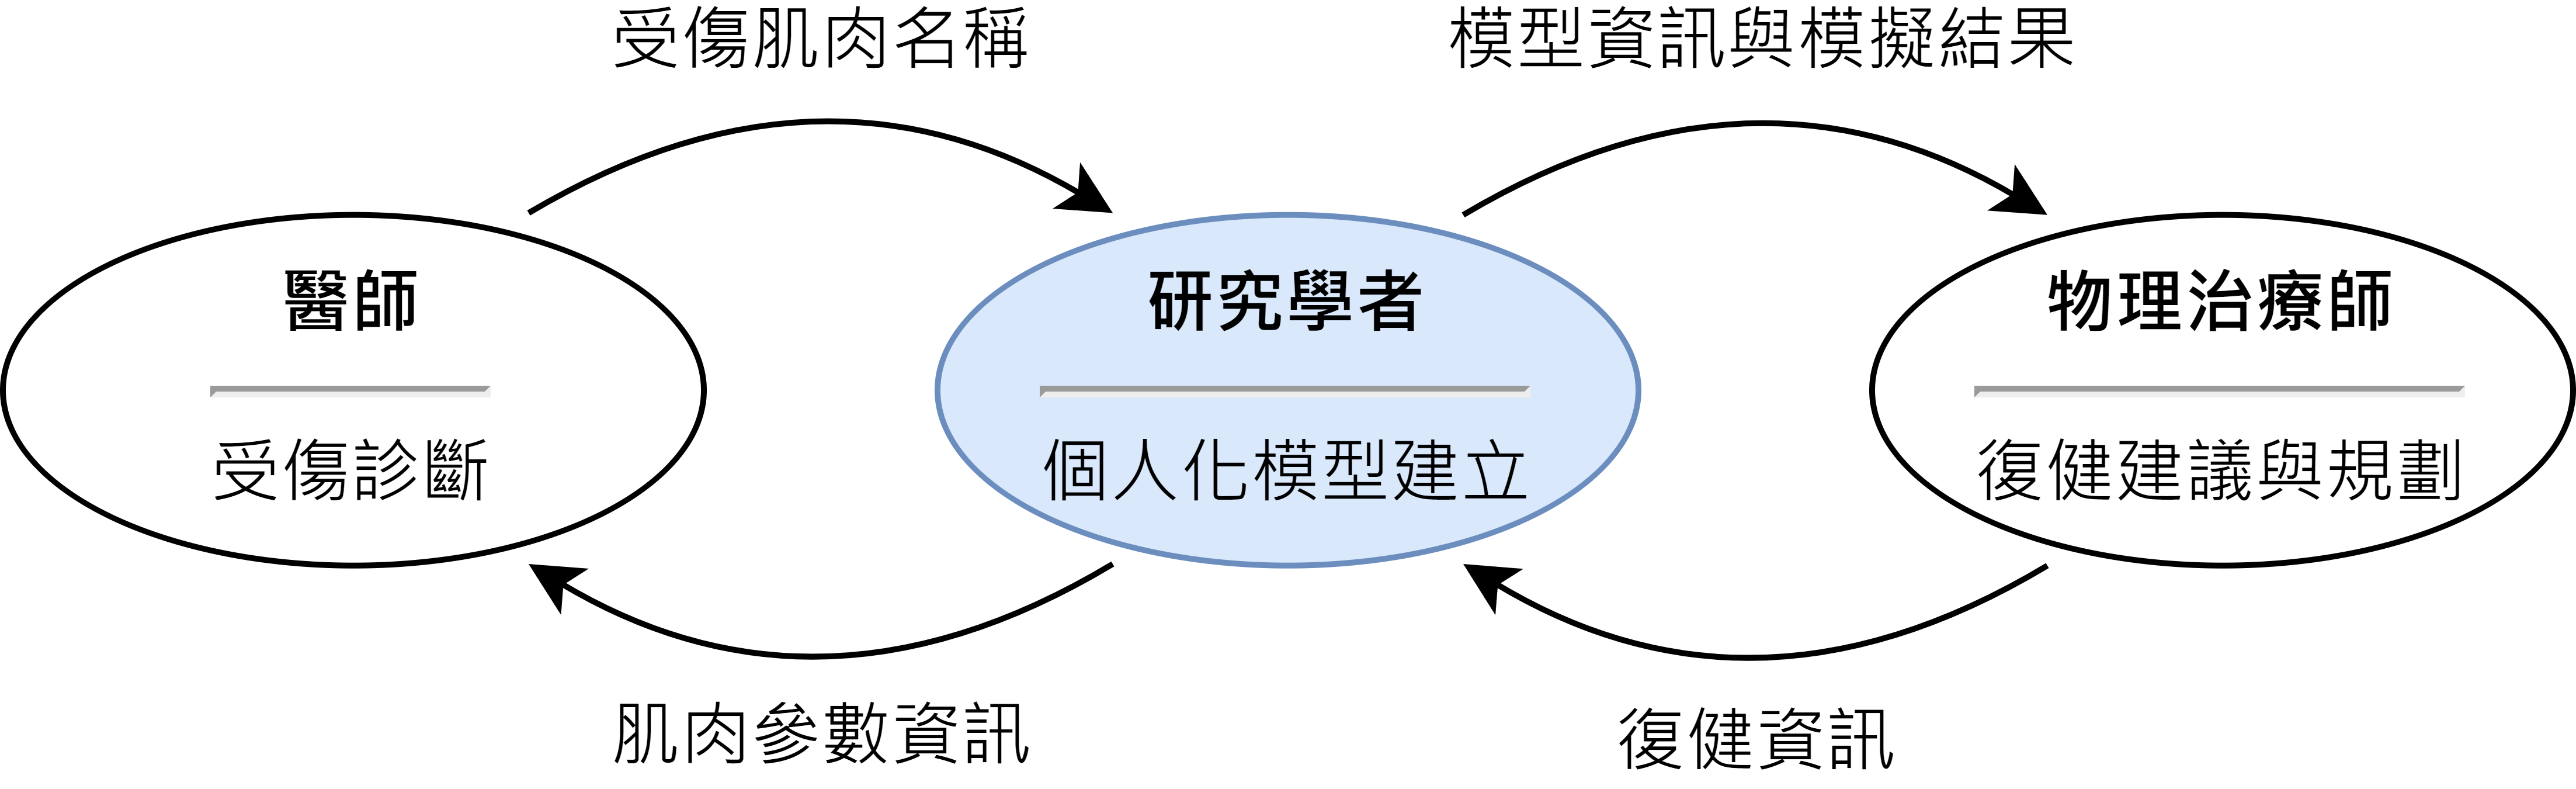
\includegraphics[width=15cm]{figure/ch1_fig_Rehab.png}
    \caption[復健規劃流程]{本研究制定之復健規劃流程,位於中間的藍色圓框為本論文之核心目標。}
    \label{ch1_fig_Rehab}
\end{figure}

% 困境;動機;目的
由於通用模型的縮放不如預期 \cite{akhundov2022subject},在居家復健的規劃中,建立個人化模型是必要的選擇,
其建立可透過醫療器材的量測,例如磁振造影 \cite{da2017feasibility} \cite{dejtiar2020development}、
超音波 \cite{sartori2017subject} \cite{passmore2017application} 等器材,但直接量測的成本相對高昂,
建立個人化模型除了常見的幾何特徵,如身高、體重、臂長等資訊外,肌肉參數也佔了重要的角色 \cite{myers2015probabilistic},
肌肉參數直接影響了肌肉的發力結果,進而關係到人體的動作與姿態,本研究目的是透過最佳化方法來評估肌肉參數,
取代傳統量測方法來建立個人化模型,但由於參數改變可由其餘參數來抗衡 \cite{bujalski2018monte},
意味著不同的參數組合能產生相似的動作結果,即所謂的參數具不可識別性 (parameter non-identifiability),
故如何提高在肌肉參數評估的準確度上,亦是本研究的主要目的之一。

% 1: 透過標準模型進行敏感度分析,找感度出不同動作所對應的高敏肌肉
% 2: 根據指定負重與動作組合 (集) 與對應的高敏感度肌肉,透過多運動軌跡預測最佳化來尋找高敏感度肌肉的參數
% 3: 提供其餘動作,作為模型驗證

\clearpage

% ------------------------- 1.3 ------------------------- %
\section{論文架構}
本論文共含有六個章節,其架構如下:

\begin{itemize}
    \item \textbf{第一章:緒論}
    \\ 介紹本論文之研究背景,由研究背景的需求與困境當中,衍生出本研究之動機與目的,闡述本論文之核心目標。
    \item \textbf{第二章:文獻回顧}
    \\ 針對該領域現存的研究進行介紹與整理,包括人體量測、模擬與分析相關研究,以及個人化模型的必要性,
    並針對肌肉參數評估等文獻,進行回顧與討論。
    \item \textbf{第三章:研究方法}
    \\ 介紹本研究所提出之參數評估方法,包含敏感度分析、參數評估與最佳化,以及模型驗證方法,
    除此之外也介紹了相關背景知識,例如肌肉模型、動力學模擬、肌肉計算控制模擬等資訊,藉由這整套方法來建立個人化模型。
    \item \textbf{第四章:上肢特定肌肉之參數評估與最佳化}
    \\ 針對第三章所提出之方法,使用普及的上肢肌肉骨骼模型作為範例,進行相關的前置作業與研究方法的套用說明。
    \item \textbf{第五章:參數評估模擬案例與成果探討}
    \\ 綜合第三章的研究方法與第四章的骨骼模型,呈現數個模擬案例來顯現該方法的有效性與必要性,
    同時驗證所評估參數之正確性,並對參數的評估結果進行探討。
    \item \textbf{第六章:結論與未來工作}
    \\ 總結本研究之成果與貢獻,並給予適當的建議,作為未來本研究之延伸方向。
\end{itemize}

\clearpage